\section{Resultate}
Sowohl in \cite{davis:2008} als auch in \cite{haller:2010} wurden zwar
vielversprechende Ansätze für Hardware-SAT-Solver vorgestellt, 
jedoch fehlen beiden Arbeiten ernstzunehmende Resultate,
da sie entweder  nur den Entwurf simulieren 
und nicht das Gesamtsystem betrachten oder ganz fehlen.
In den folgenden Abschnitten werden Resultate des
vorgestellen Enwurfs diskutiert.

\subsection{Synthese des Entwurfs}
Zur Umsetzung des Entwurfes stand ein Xilinx ML505
Entwicklerboard \cite{xilinxml505:2011} mit einem Virtex-5
XC5VLX50T FPGA \cite{xilinxvirtex5:2009} zur Verfügung .
Für den Entwurf wurde die Ethernet PHY Schnittstelle und
der FPGA auf dem Entwicklerboard benutzt.
Auf dem FPGA-Chip sind 7200 Logikzellen mit je 4 LUTs und FlipFlops, 
60 x 36\,kbit Block-RAM (oder 120 x 18\,kbit),
480 kbit Distributed-RAM und 4 Ethernet-MACs vorhanden.\\
Für diesen FPGA kann ein Entwurf mit 32 Propagation-Engines, 128 Klauseln in 9 SAT pro
Propagation Engine und 256 Variablen synthetisiert werden. Der Schaltkreis wird mit
125\,MHz getaktet. Man könnte ihn sogar noch höher takten (ca. 250\,MHz), jedoch wurde zwecks einfacher
Kommunikation mit dem Ethernetmodul darauf verzichtet.
Die Synthese wurde mithilfe von ISE in Version 10.1.02 (lin64) durchgeführt.
Eine Zusammenfassung über die benötigten Ressourcen des synthetisierten Schaltkreises findet man in 
Tabelle \ref{ressources}.
\begin{table}[h]
  \begin{tabular}{|l|l|l|l|}
    \hline
    \textsc{Logikelement} & \textsc{Benutzt} & \textsc{Verfügbar} &\textsc{Ausnutzung}\\
    \hline
    \hline
    LUTs & 10053 & 28800 & 34\%\\
    \hline
    davon LUTs als Logik & 8348 & - & -\\
    \hline
    davon LUTs als Speicher & 1698 & - & -\\
    \hline
    FlipFlops & 5701 & 28800 & 19\%\\
    \hline
    Block-RAM & 53 & 60 & 88\%\\
    \hline
    davon 18\,Kbit Block-RAM & 70 & - & -\\
    \hline
    davon 36\,Kbit Block-RAM & 18 & - & -\\
    \hline
  \end{tabular}
  \caption{Ressourcenverbrauch des Entwurfs auf Virtex 5 X50T}
  \label{ressources}
\end{table}
Der Flaschenhals des Entwurfs liegt eindeutig im Verbrauch von Block-RAM.
Die 32 Propagation-Engines brauchen 64 x 18\,kbit Block-RAM und die
restlichen 18 x 36\,kbit und 6 x 18\,kbit Block-RAMs werden vom 
Literal-Übersetzungs-Modul benutzt. Die Lookup-Tabellen des FPGAs sind
nur zu 34\% ausgelastet, so dass noch viel Platz für Logik vorhanden ist
und auch die FlipFlops der LUTs sind nur mäßig belegt.


\subsection{Experimente}
In diesem Unterkapitel soll der in dieser Arbeit entstandene 
FPGA-SAT-Solver mit einem Software-Solver verglichen werden.
Der Software-Solver ist ein reiner DPLL-Solver und 
verhält sich exakt so wie der FPGA-Solver. 
Das heißt, es werden die gleichen Entscheidungen getroffen
und bei Konflikten wird der gleiche Rücksprungpunkt bestimmt,
so dass die Solver den gleichen Suchbaum erzeugen.
Nur die benutzten Algorithmen zur 
Umsetzung des Inferenzprozesses sind unterschiedlich.
Der Software-Solver sucht im Inferenzprozess jede Klausel
nach möglichen Unit-Literalen ab.\\
Um die Unterschiede zwischen Software- und 
Hardware-SAT-Solver zu verdeutlichen wurden
drei Testfälle ausgewählt:
\begin{itemize}
  \item 
    \textbf{Testfall 1} besteht aus einer Menge von Formeln mit maximal 32 Klauseln,  
    welche durch das Propagieren von Literal $l = -1$ gleichzeitig Unit werden und somit 
    den Inferenzprozess anstoßen. Mehr als 32 Klauseln können nicht
    gleichzeitig getestet werden, da der FPGA nur bis zu 32
    Gruppen unterstützt. Dieser Test wurde ausgewählt um die parallele Leistungsfähigkeit
    der Solver zu testen.
  \item
    \textbf{Testfall 2} besteht aus einer Menge von Formeln mit maximal
    100 Klauseln, wobei durch Propagieren von Literal $l = -1$ eine
    Inferenzkette von Unit-Literalen entsteht.
    Mit diesem Test wird geprüft wie die Leistungsfähigkeit die Solver bei
    der seriellen Abarbeitung von Literalen sind.
  \item
    \textbf{Testfall 3} besteht aus ausgewählten Instanzen
    der SATLIB \cite{satlib:2003} und einer kleinen Instanz der SAT-Competition \cite{satcomp:2011}. 
    Diese Probleme wurden ausgewählt, um die Leistung der Solver
    bei bereits vorhandenen Problemen zu vergleichen.
\end{itemize}
Im getesteten System sollen alle Faktoren mit
eingerechnet werden. So werden auch die 
Ethernetübertragungszeiten nicht vernachlässigt, da
sie einen Großteil der benötigten Zeit stellen.
Die Zeit die der FPGA benötigt, um ein Literal
zu propagieren ist fast vernachlässigbar. Er braucht
genau 76 Takte, dass entspricht 608\,ns bei
einer Taktfrequenz von 125\,MHz. In den 76 Takten 
sind bereits die Ethernetverabeitungszeiten
enthalten. Für das Senden eines Pakets muss
man dann nocheinmmal ca. 300\,$\mu$s veranschlagen.
In den Experimenten 1 bis 3 werden jeweils
die Anzahl der gesendeten Pakete angegeben.
Außerdem muss bedacht werden, dass
die Software des Host-PCs auch noch 
Zeit braucht. Diese Zeit ist jedoch schwer
zu bestimmen, da sie von der momentanen Auslastung
des Hostsystems abhängt. Der bei den Experimenten
genutzte Host-PC ist ein Intel Core 2 Quad 2.6\,GHz 
64\,Bit mit 8\,Gbyte Hauptspeicher.



\subsubsection{Parallele Inferenz von Literalen}
In diesem Testfall soll die parallele Leistung
von Software- und Hardware-SAT-Solver gemessen
werden, um zu zeigen, welche Auswirkungen die
verschiedenen Inferenzalgorithmen auf
das Zeitverhalten haben. Es wurden 9 Formeln 
mit jeweils 1, 4, 8, 12, 16, 20 , 24, 28 und 32
Klauseln ausgewählt. Diese Klauseln werden Unit wenn das Literal
$l = -1$ propagiert wird, wobei alle Unit-Literale unterschiedlich sind.
\begin{center}
      $F_{Test1\ [32]} = \langle [1,2],[1,3],...,[1,32],[1,33]\rangle$
\end{center}
In der Laufzeit des FPGA Solvers werden 
3 Ethernetpakete verschickt (Initialisierungs-, Entscheidungs-,
Eingabepaket).
Das Zeitverhalten in Abhängigkeit von
der Anzahl der Klauseln wird in Abbildung \ref{parallelinferenz}
grafisch dargestellt.
\begin{figure}[h]
  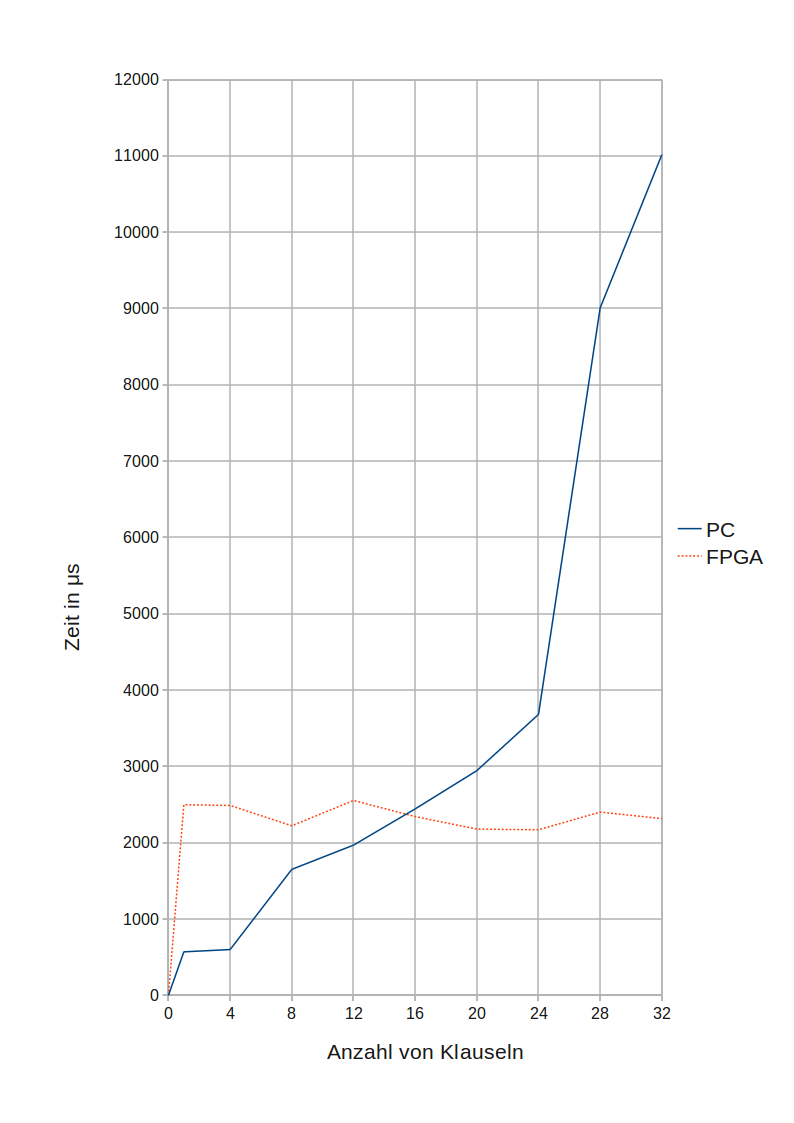
\includegraphics[width=0.65\textwidth]{abb/testfall1.png}
  \caption{Parallele Inferenz von Literalen}
  \label{parallelinferenz}
\end{figure}
Man erkennt in Abbildung \ref{parallelinferenz} gut, dass obwohl sich
die Anzahl der Klauseln erhöht, die Zeit welche der FPGA-SAT-Solver benötigt, 
um die Formel zu lösen, stets konstant bleibt. Diese Eigenschaft lässt sich
leicht erklären. Da alle 32 Propagation-Engines parallel arbeiten und sich
alle Klauseln in verschiedenen Gruppen befinden, können auch alle
Klauseln gleichzeitig propagiert werden.
Im Schnitt benötigt der FPGA Solver also 2,5\,ms, wovon 0,9\,ms auf das
Versenden von Paketen zurückzuführen sind. Die restliche Zeit
benötigt der Host-PC für seine Berechnungen.\\
Im Gegensatz dazu steigt die benötigte Zeit des Software Solvers
mit zunehmender Klauselanzahl stark an. Dies 
ist darauf zurückzuführen, dass der Software-Solver
Literale nicht parallel verarbeiten kann.

\subsubsection{Serielle Inferenz von Literalen}
Auch die serielle Leistung der Solver muss verglichen werden.
Hierfür eignet sich eine Formel mit Inferenzkette. Das heißt, jedes
Unit-Literal erzeugt in einer anderen Klausel wiederum ein Unit-Literal und so weiter.
Es wurden 8 Formeln mit jeweils 1, 4, 8, 16, 32, 64, 80 und
100 Klauseln getestet. 
    \begin{center}
      $F_{Test2} = \langle [1,2],[-2,3],[-3,4],[-4,5][-5,6],...,[-100,101]\rangle$\\
      $Inferenzkette:\ \ \ \ \ \ \ -1 \rightarrow 2 \rightarrow 3 \rightarrow 4 \rightarrow ... \rightarrow 100 \rightarrow 101$
    \end{center}
Für die Formeln mit 1 bis 64 Klauseln
werden 3 Pakete für den FPGA Solver benötigt (Initialisierungs-, Entscheidungs-, Eingabepaket).
Die Formeln mit 80 bzw. 100 Klauseln benötigen 1 Paket
mehr, da die Formel nicht mehr allein in ein Initialisierungspaket passt.
\begin{figure}[h]
  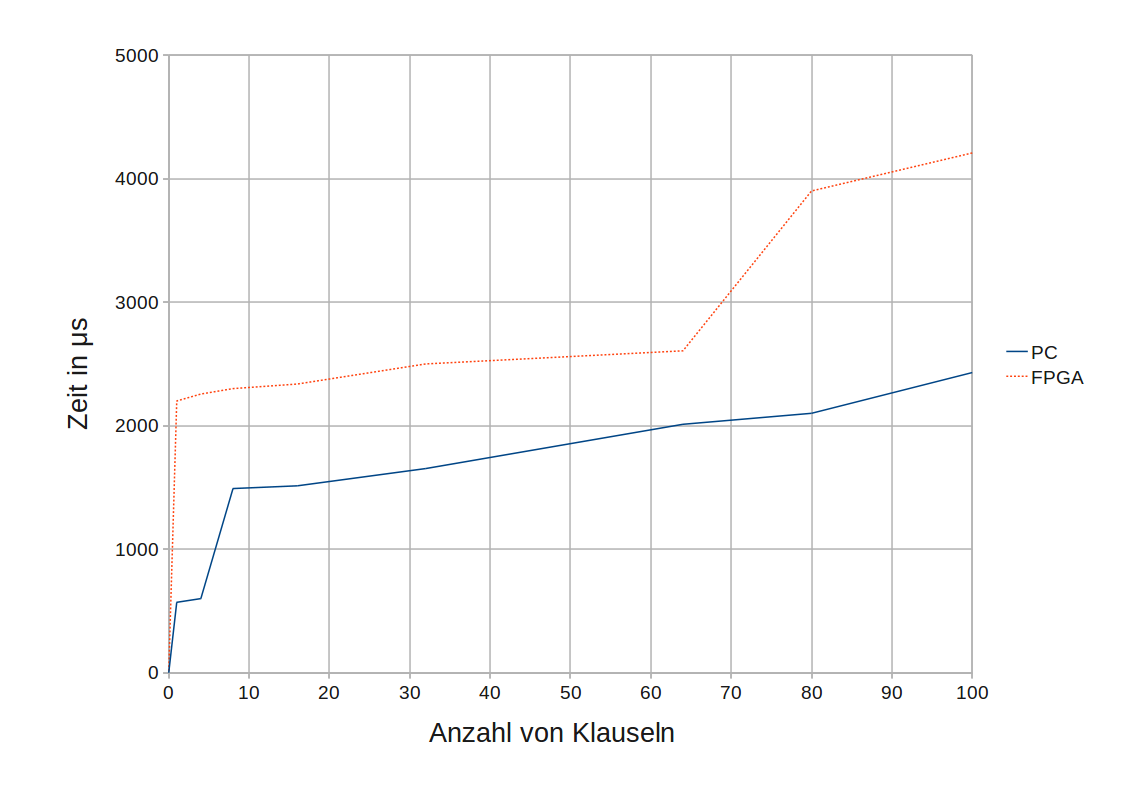
\includegraphics[width=\textwidth]{abb/testfall2.png}
  \caption{Serielle Inferenz von Literalen}
  \label{seriellinferenz}
\end{figure}
In Abbildung \ref{seriellinferenz} ist zu erkennen, dass der FPGA-Solver stets mehr
Zeit benötigt als die Software-Lösung. Der Zeitanstieg in
Abhängigkeit zur Anzahl von Klauseln ist jedoch gleich. Der PC ist zwar
mehr als 10 mal so hoch getaktet wie der FPGA, jedoch braucht der
FPGA weniger als ein Zehntel der Zeit, um ein Literal zu propagieren.
Somit gleichen sich Hardware- und Softwarelösung im seriellen Vergleich
aus. Für die größeren Lösungszeiten sorgt letztendlich nur
die Ethernetkommunikation. Ab 80 Klauseln benötigt der FPGA-Solver
plötzlich mehr Zeit. Diese Zeit ist auf das zusätzliche
Ethernetpaket zurückzuführen, welches gesendet werden muss.


\subsubsection{Lösen von ausgewählten Problemen}
Natürlich bestehen SAT-Probleme nicht nur aus paralleler
bzw. serieller Inferenz sondern aus einer Mischung von
beidem. Dazu kommt noch, dass die Entscheidungsheuristik
eines SAT-Solvers nicht immer richtig liegt und der
Suchprozess früher oder später in einem Konflikt endet.
Um Konflikte zu lösen, muss der FPGA-SAT-Solver wieder
Pakete verschicken, wobei sich gezeigt hat, dass sich dies
negativ auf die Laufzeiten auswirkt.
\begin{table}[h]
  \centering
  \begin{tabular}{|l|l|l|l|}
    \hline
    \textsc{Instanz} & \textsc{Variablen} & \textsc{Klauseln} &\textsc{Gruppen}\\
    \hline
    \hline
    anomaly.cnf & 48 & 261 & 22\\
    \hline
    flat-easy-1.cnf & 90 & 300 & 8\\
    \hline
    289-sat-4x8.cnf & 128 & 896 & 25\\
    \hline
  \end{tabular}
  \caption{Daten ausgewählter Probleme}
  \label{problems_data}
\end{table}
Anhand von SAT-Instanzen aus der SATLIB \cite{satlib:2003} und
SAT-Competition \cite{satcomp:2011}
sollen Hardware- und Software-Solver unter realen 
Bedingungen verglichen werden. Bei den Instanzen handelt es
sich um ein Planungsproblem (Blocks World:anomaly.cnf), 
ein Graphfärbeproblem (Graph Coloring:Flat Easy:flat-easy-1.cnf) 
und ein Problem unbekanntem Typs (289-sat-4x8.cnf).
In Tabelle \ref{problems_data} werden Eigenschaften der Problemdateien
aufgelistet. Ergebnisse findet man in Tabelle \ref{problems}. Wobei die Laufzeiten
Durschnittswerte aus mehreren Durchläufen sind.
\begin{table}[h]
  \centering
  \begin{tabular}{|l|l|l|l|l|}
    \hline
    \textsc{Instanz} & \textsc{Laufzeit PC} & \textsc{Laufzeit FPGA} &\textsc{ges. Pakete}&\textsc{Sendezeit}\\
    \hline
    \hline
    anomaly.cnf & 6,1\,ms & 10,2\,ms & 17 & 5,1\,ms\\
    \hline
    flat-easy-1.cnf & 8,2\,ms & 22,0\,ms & 53 & 15,9\,ms\\
    \hline
    289-sat-4x8.cnf & 22,6\,ms & 60,7\,ms & 129 & 38,7\,ms\\
    \hline
  \end{tabular}
  \caption{Ergebnisse ausgewählter Probleme}
  \label{problems}
\end{table}
\newpage
Dabei werden folgende Instanzen unterschieden:
\begin{itemize}
  \item
    \textbf{anomaly.cnf}\\
    Das Problem lässt sich in 22 Gruppen gruppieren und kann somit vom FPGA-Solver
    gelöst werden. Er braucht 10,237\,ms und somit ca. 4\,ms mehr als der Software
    Solver. Die Ethernetsendezeit beträgt 5,1\,ms und somit die Hälfte der gesamten
    Laufzeit.

  \item
    \textbf{flat-easy.cnf}\\
    Für dieses Problem werden nur 8 Gruppen benötigt und es kann somit auch ohne weiteres
    vom FPGA-Solver gelöst werden. Es müssen 53 Ethernetpakete zur Kommunikation
    zwischen Host und FPGA verschickt werden. Das sind wesentlich mehr als bei
    anomaly.cnf, was sich auf die Laufzeit des FPGA-Solvers auswirkt. Die Softwarelösung
    benötigt 14\,ms weniger Zeit als der FPGA, wobei 15,9\,ms der FPGA-Lösungszeit
    von der Paketsendung verbraucht wird.
\item
    \textbf{289-sat-4x8.cnf}\\
    Bei dieser Problemdatei handelt es sich um die größte Formel der
    ausgewählten Instanzen. Zieht
    man von der Lösungszeit des FPGA-Solvers die Zeit, welche
    für das versenden der Pakete gebraucht wird ab, dann lösen
    beide Solver die Problemdatei in der gleichen Zeit.

\end{itemize}
\subsection{Fazit}
In diesem Abschnitt sollen nochmal alle Testfälle zusammengefasst
werden, um daraus ein Fazit ziehen zu können. So hat sich durch
Testfall 1 gezeigt, dass der FPGA-SAT-Solver Literal besser
parallel verarbeiten kann, denn Literale werden in den einzelnen
Gruppen alle gleichzeitig propagiert. Bei der seriellen Inferenz, 
in Testfall 2, schneiden FPGA- und Software-SAT-Solver etwa gleich ab, wobei
der FPGA-Solver mit einem Ethernet-Overhead zu kämpfen hat.
Parallele und serielle Inferenz wurden in Testfall 3 bei
realen Problemen sozusagen gemischt. Bei allen Problemen
ist der Software-Solver klar schneller, da der Solver nicht 
mit einem FPGA kommunizieren muss. Der FPGA-SAT-Solver konnte
jedoch nicht sein volles Potential ausschöpfen, weil
es schwierig ist große Formel zu finden,
welche, trotz der vielen Beschränkungen, lösbar sind. Denn selbst
wenn Variablen und Klauselanzahl unter den Möglichkeiten bleiben, 
muss es nicht gezwungenermaßen möglich sein, 
eine Gruppierung für 32 Gruppen durchzuführen.
Bei allen Problemdateien könnte der FPGA-Solver,
durch eine schnellere Kommunikation zum Host-PC, an die Lösungszeiten
des Software-Solvers herankommen.
Denn bei geringerer Kommunikationlatenz oder
besserer Verschränkung der Kommunikation zwischen FPGA und Host-PC, ist eine
Verbesserung der Lösungszeit
durchaus denkbar. 
Einen klaren Vorteil hat die Software-Lösung
in Hinsicht auf die Problemgröße der SAT-Instanzen. Dem 
Software-Solver steht ein großer DRAM-Speicher zur Verfügung, welcher
wesentlich mehr als 256 Variablen und 4096 Klauseln zulässt.\\
Schlussendlich kann man sagen, das der Software-Solver
bei den getesteten Problemen stets die bessere Wahl ist. Jedoch
gibt es Möglichkeiten Performance und Ressourcenausnutzung
des FPGA-SAT-Solvers zu verbessern. Einige dieser Möglichkeiten werden im
folgenden Abschnitt näher betrachet.






